% This is appendix-frames.tex of the OpenMP specification.
% This is an included file. See the master file for more information.
%
% When editing this file:
%
%    1. To change formatting, appearance, or style, please edit openmp.sty.
%
%    2. Custom commands and macros are defined in openmp.sty.
%
%    3. Be kind to other editors -- keep a consistent style by copying-and-pasting to
%       create new content.
%
%    4. We use semantic markup, e.g. (see openmp.sty for a full list):
%         \code{}     % for bold monospace keywords, code, operators, etc.
%         \plc{}      % for italic placeholder names, grammar, etc.
%
%    5. Other recommendations:
%         Use the convenience macros defined in openmp.sty for the minor headers
%         such as Comments, Syntax, etc.
%
%         To keep items together on the same page, prefer the use of
%         \begin{samepage}.... Avoid \parbox for text blocks as it interrupts line numbering.
%         When possible, avoid \filbreak, \pagebreak, \newpage, \clearpage unless that's
%         what you mean. Use \needspace{} cautiously for troublesome paragraphs.
%
%         Avoid absolute lengths and measures in this file; use relative units when possible.
%         Vertical space can be relative to \baselineskip or ex units. Horizontal space
%         can be relative to \linewidth or em units.
%
%         Prefer \emph{} to italicize terminology, e.g.:
%             This is a \emph{definition}, not a placeholder.
%             This is a \plc{var-name}.
%


\chapter{Interaction Diagram of OMPD Components}
\index{ompd diagram}
\label{chap:ompd_diagram}


   \begin{figure}[h]
    \centering
        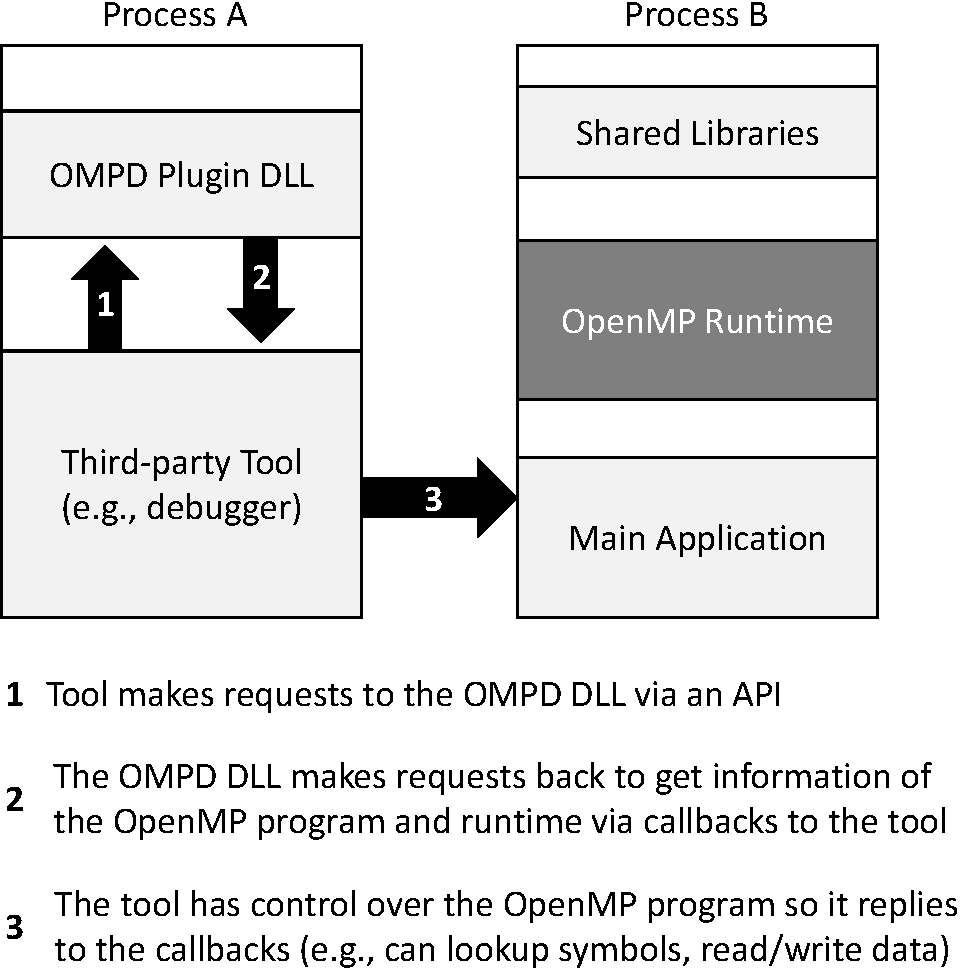
\includegraphics[width=3.5in]{appendices/ompd_diagram.pdf}
    \caption{Interaction Diagram of OMPD Components}
    \label{fig:ompd_diagram}
\end{figure}

The figure shows how the different components of OMPD fit together. The third-party tool loads
the OMPD library
that matches the OpenMP runtime being used by the OpenMP program. The
library exports the API defined in
\specref{sec:ompd-overview}, which the tool uses to get
OpenMP information about the
OpenMP program. The OMPD
library will need to look up the symbols, or read data out of the
OpenMP program. It does not do this directly,
but instead asks the tool to perform these operations
for it using a callback interface exported
by the tool.

This architectural layout insulates the tool from the details of the
internal structure of the
OpenMP runtime. Similarly, the OMPD library does not need to be
concerned about how to access
the OpenMP program. Decoupling the library and tool in this
way allows for flexibility in how the OpenMP program and tool are deployed, so that, for example,
there is no requirement that tool and OpenMP program
execute on the same machine.

\crossreferences
\begin{itemize}
\item See \specref{sec:ompd-overview}.
\end{itemize}

